\documentclass[11pt,a4paper]{article}

% --- Core Packages ---
\usepackage[utf8]{inputenc}
\usepackage[T1]{fontenc}
\usepackage[margin=1in,bottom=1.2in]{geometry}
\setlength{\headheight}{24pt}
\addtolength{\topmargin}{-12pt}
\usepackage{helvet}
\renewcommand{\familydefault}{\sfdefault}
\usepackage{xcolor}
\usepackage{graphicx}
\usepackage{fancyhdr}
\usepackage{titlesec}
\usepackage{hyperref}
\usepackage{tcolorbox}
\usepackage{booktabs}
\usepackage{lastpage}
\usepackage{tikz}
\usetikzlibrary{shadows,calc}

% --- Modern Color Palette ---
\definecolor{primaryGold}{HTML}{D4AF37}
\definecolor{deepBlack}{HTML}{0A0A0A}
\definecolor{lightGray}{HTML}{F5F5F5}
\definecolor{accentBlue}{HTML}{0052FF}

% --- Header and Footer Styling ---
\pagestyle{fancy}
\fancyhf{}
\renewcommand{\headrulewidth}{0.4pt}
\renewcommand{\headrule}{\hbox to\headwidth{\color{primaryGold}\leaders\hrule height \headrulewidth\hfill}}

\fancyhead[L]{\textcolor{deepBlack}{\textbf{BotIn Technical Specification}}}
\fancyhead[R]{\textcolor{primaryGold}{\textit{Protocol Standards}}}

\fancyfoot[L]{\scriptsize \textit{2026 \copyright \ \textbf{c0bw3b Inc.} All Rights Reserved. \texttrademark \ | Llakterian @ c0bw3b Inc.}}
\fancyfoot[R]{\scriptsize \textcolor{gray}{\thepage\ / \pageref{LastPage}}}

% --- Section Styling ---
\titleformat{\section}
  {\color{deepBlack}\normalfont\Large\bfseries}
  {\thesection}{1em}{}[{\titlerule[0.8pt]\vspace{2pt}\color{primaryGold}\titlerule[1.5pt]}]

\titleformat{\subsection}
  {\color{deepBlack}\normalfont\large\bfseries}
  {\thesubsection}{1em}{}

% --- Custom Boxes ---
\newtcolorbox{premiumbox}[1]{
  colback=lightGray,
  colframe=primaryGold,
  fonttitle=\bfseries,
  title=#1,
  enhanced,
  drop shadow,
  sharp corners=southwest
}

\begin{document}

\begin{center}
    \vspace*{1.5cm}
    {\Huge \textbf{\textcolor{deepBlack}{Technical Specification}}} \\
    \vspace{0.5cm}
    {\Large \textcolor{primaryGold}{BotIn Protocol Standards}} \\
    \vspace{1.5cm}
    \begin{tikzpicture}
        \draw[fill=lightGray, draw=primaryGold, line width=1pt, drop shadow] (0,0) rectangle (8,3.5);
        \node at (4,2.8) {\textbf{Technical Lead}};
        \node at (4,2.2) {\textcolor{accentBlue}{BotIn Specification}};
        \node at (4,1.6) {\scriptsize \textcolor{gray}{c0bw3b Ecosystem Documentation}};
        \node at (4,0.8) {\small \textbf{Version: 1.0.0}};
    \end{tikzpicture}
    \vspace{1.5cm}
\end{center}

\section{Executive Summary}
BotIn is a cutting-edge decentralized protocol architected to facilitate sovereign identity, trustless reputation, and autonomous economic interaction for AI agents.

\section{Protocol Standards}

\subsection{1. ERC-8004: Trustless Agent Framework}
BotIn is built upon the ERC-8004 standard, which defines lightweight on-chain registries for agent discovery and validation.

\subsection{2. ERC-4337: Account Abstraction (AA)}
We utilize ERC-4337 to decouple agent logic from gas management through smart accounts and paymasters.

\section{Core Smart Contracts}
\begin{itemize}
    \item \textbf{BotInIdentityRegistry.sol:} The sovereign source of truth for network participants.
    \item \textbf{BotInPaymentVault.sol:} The pecuniary engine orchestrating automated subscriptions.
    \item \textbf{BotInReputationRegistry.sol:} The decentralized trust layer with optimized data structures.
\end{itemize}

\section{Frontend Architecture}
\begin{itemize}
    \item \textbf{Framework:} React 18 / Vite / TypeScript.
    \item \textbf{Connectivity:} Wagmi v2 + Viem.
    \item \textbf{Identity Resolution:} IPFS focused metadata persistence.
\end{itemize}

\section{Security and Integrity}
\begin{itemize}
    \item \textbf{Logic Safety:} Checks-Effects-Interactions pattern for reentrancy mitigation.
    \item \textbf{Access Control:} Granular RBAC via OpenZeppelin.
\end{itemize}

\end{document}
